\chapter{Critical Exploration of the Data}
For exploring the data properly, we divide the data into two groups: one being categorical and the other being numerical. 

\begin{itemize}
    \item Here, categorical features are defined if the the attribute has less than 6 unique elements else it is a numerical feature.
    \item Typical approach for this division of features can also be based on the datatypes of the elements of the respective attribute.

    Eg : datatype = integer, attribute = numerical feature ; datatype = string, attribute = categorical feature
    \item For this dataset, as the number of features are less, we can manually check the dataset as well.    
\end{itemize}

After analyzing the data-types completely, we come to the conclusion:
\begin{listing}[!htpb]
\inputminted{octave}{Code/f1.m}
\end{listing}
\newpage 

\section{Distribution of the categorical features}
% \begin{longlisting}
% \inputminted{octave}{Code/f2.m}
% \end{longlisting}
\begin{figure}[!htpb]
    \centering
    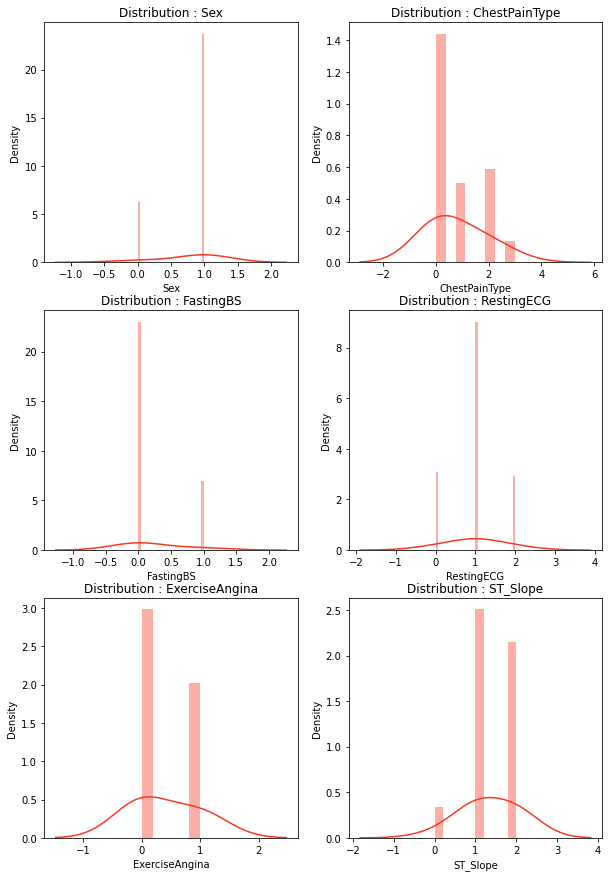
\includegraphics[width=0.6\linewidth]{Figures/Outputs/distr-of-catf.png}
    \label{Distribution of all categorical features}
    \caption{Distribution of all the categorical features.}
\end{figure}

And the distribution of heart diseases according to gender is:
\begin{figure}[!htpb]
    \centering
    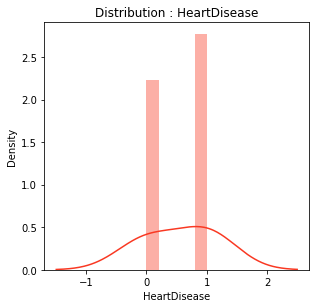
\includegraphics[width=0.3\linewidth]{Figures/Outputs/distr-of-catf2.png}
    \label{Distribution of heart diseases according to gender.}
    \caption{Distribution of heart diseases according to gender}
\end{figure}

We deduce that all the categorical features are nearly \textbf{normally distributed}.
\newpage 
\section{Distribution of all the numerical features}
\begin{figure}[!htpb]
    \centering
    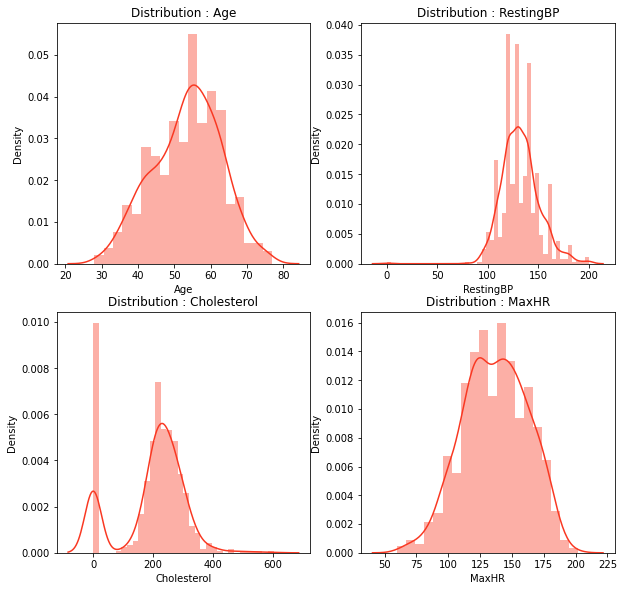
\includegraphics[width=0.7\linewidth]{Figures/Outputs/dist-num-1.png}
    \label{Distribution of all numerical features}
    \caption{Distribution of all numerical features.}
\end{figure}
\begin{figure}[!htpb]
    \centering
    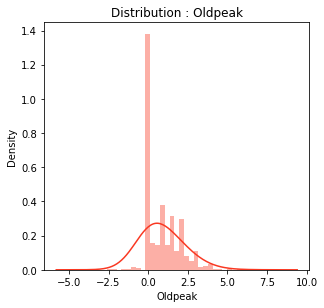
\includegraphics[width=0.3\linewidth]{Figures/Outputs/dist-num-2.png}
    \label{Distribution of oldpeak}
    \caption{Distribution of oldpeak.}
\end{figure}

We deduce that 
\begin{itemize}
    \item \textbf{Oldpeak's} data distribution is rightly skewed.
    \item \textbf{Cholestrol} has a bi-modal data distribution. 
\end{itemize}
\newpage 
\section{Target visualization of heart diseases}
\begin{figure}[!htpb]
    \centering
    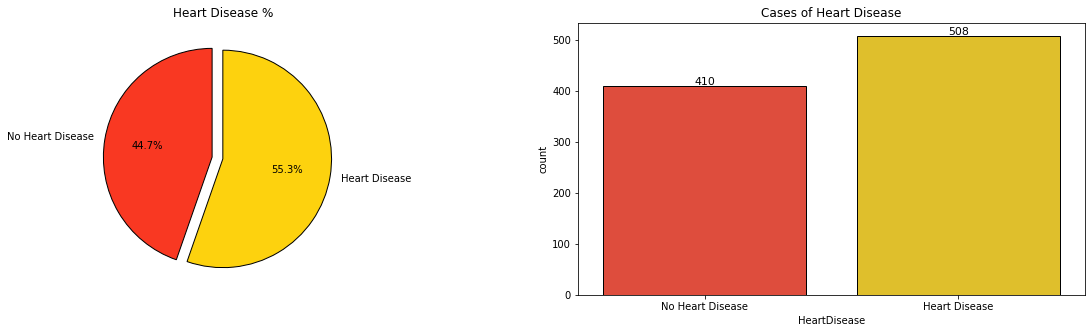
\includegraphics[width=\linewidth]{Figures/Outputs/target-visualization.png}
    \label{Visulazation of target}
    \caption{Visualization of percentage of diseased vs non-diseased candidates in the dataset.}
\end{figure}
We find that the data-set is pretty much \textbf{evenly balanced}.

\section{Comparison of Categorical Features against heart failures}
\begin{figure}[!htpb]
    \centering
    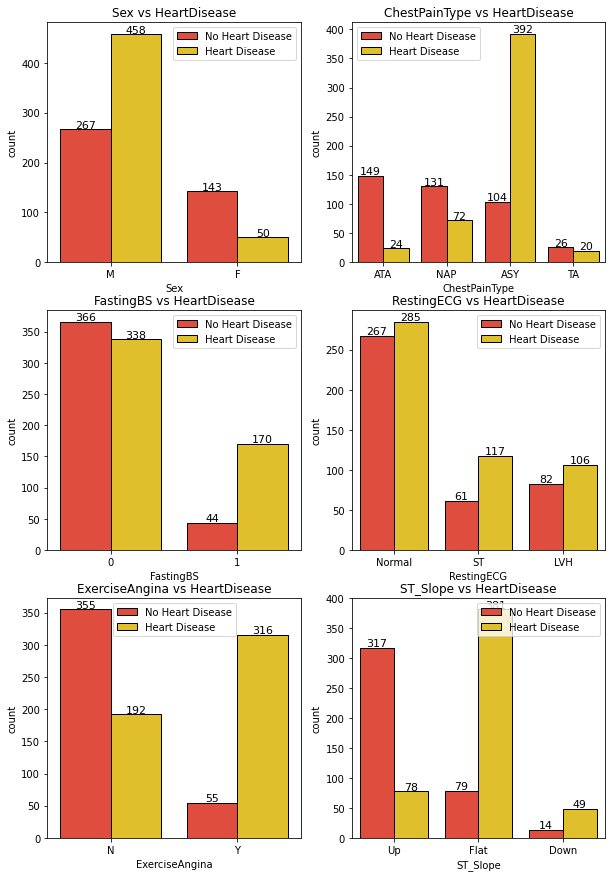
\includegraphics[width=0.5\linewidth]{Figures/Outputs/cat-vs-tar.png}
    \label{Comparison between categorical features against heart failures}
    \caption{Comparison of categorical features against diseased candidates}
\end{figure}
\subsection*{Conclusions}
\begin{itemize}
    \item \textbf{Male} population has more heart disease patients than no heart disease patients. In the case of \textbf{Female} population, heart disease patients are less than no heart disease patients. 
    \item \textbf{ASY} type of chest pain boldly points towards major chances of heart disease.
    \item \textbf{Fasting Blood Sugar} is tricky! Patients diagnosed with Fasting Blood Sugar and no Fasting Blood Sugar have significant heart disease patients. 
    \item \textbf{RestingECG} does not present with a clear cut category that highlights heart disease patients. All the 3 values consist of high number of heart disease patients.
    \item \textbf{Exercise Induced Angina} definitely bumps the probability of being diagnosed with heart diseases.
    \item With the \textbf{ST\_Slope} values, \textbf{flat} slope displays a very high probability of being diagnosed with heart disease. \textbf{Down} also shows the same output but in very few data points. 
\end{itemize}

\section{Categorical Features against Positive Heart Disease Cases}
\begin{figure}[!htpb]
    \centering
    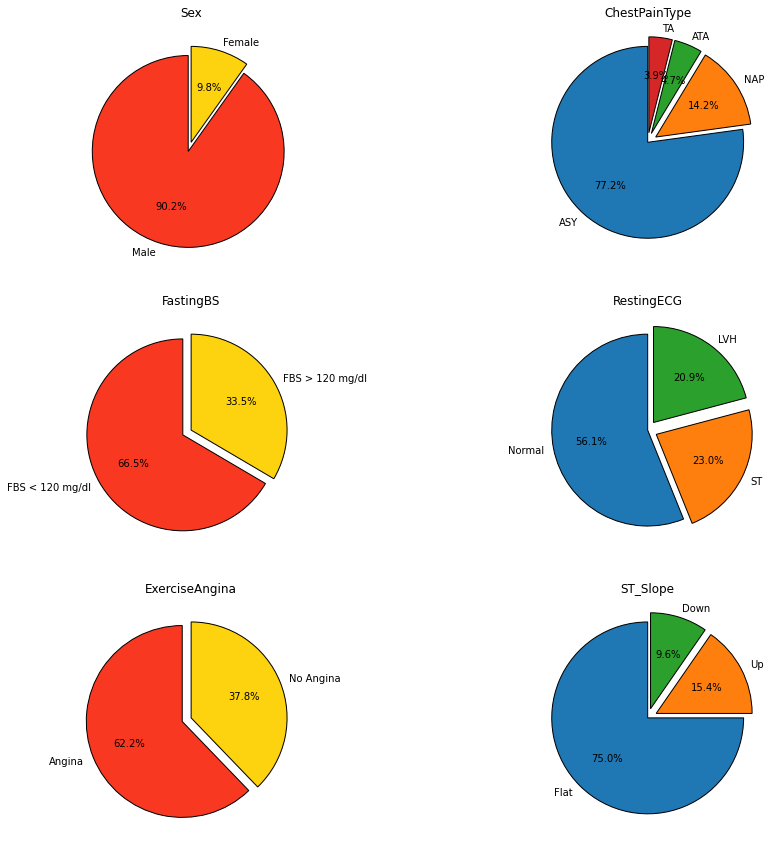
\includegraphics[width=0.5\linewidth]{Figures/Outputs/cat-pos-dis.png}
    \label{Comparison between categorical features against true cases of heart diseases}
    \caption{Comparison of categorical features against the positive cases of heart diseases.}
\end{figure}

\subsection*{Conclusion}
\begin{itemize}
    \item Out of all the heart disease patients, a staggering 90\% patients are \textbf{male}.
    \item When it comes to the type of chest pain, \textbf{ASY} type holds the majority with 77\% that lead to heart diseases.
    \item \textbf{Fasting Blood Sugar} level < 120 mg/dl displays high chances of heart diseases.
    \item For \textbf{RestingECG}, \textbf{Normal} level accounts for 56\% chances of heart diseases than \textbf{LVH} and \textbf{ST} levels.
    \item Detection of \textbf{Exercise Induced Angina} also points towards heart diseases.
    \item  When it comes to \textbf{ST\_Slope} readings, \textbf{Flat} level holds a massive chunk with 75\% that may assist in detecting underlying heart problems. 
\end{itemize}

\section{Numerical Features against Heart Diseases}
\begin{figure}[!htpb]
    \centering
    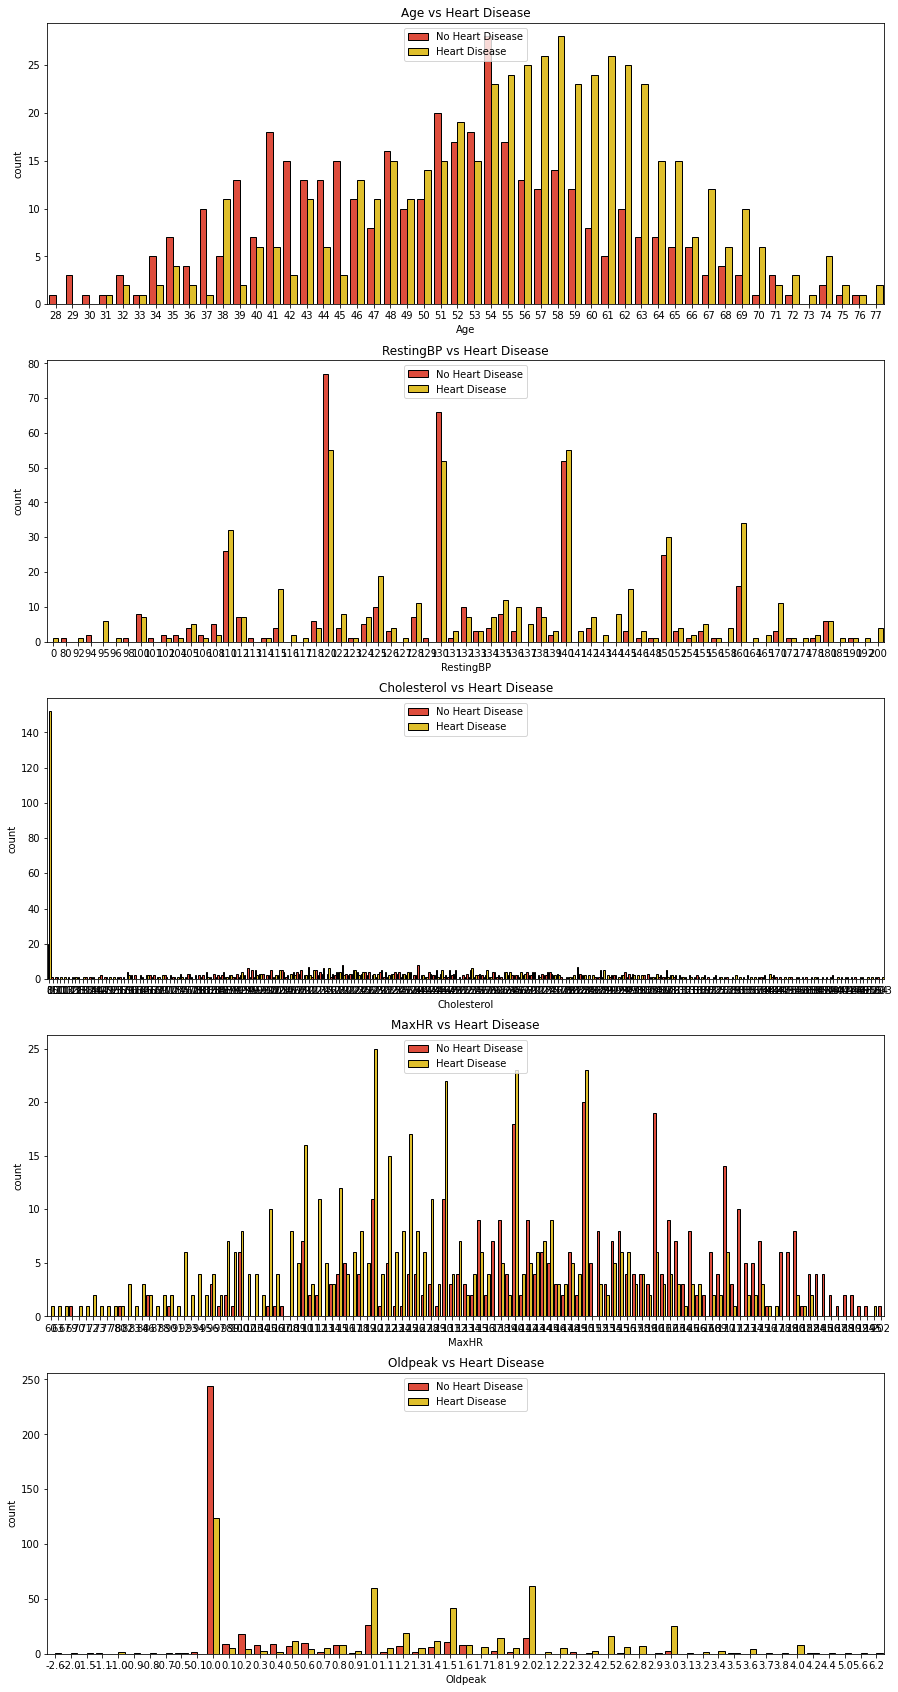
\includegraphics[width=0.4\linewidth]{Figures/Outputs/num-tar-var.png}
    \label{Comparison between numerical features and Heart Diseases}
    \caption{Comparison of numerical features against the positive cases of heart diseases.}
\end{figure}

Because of too many unique data points in the above features, it is difficult to gain any type of insight. Thus, we will convert these numerical features,except age, into categorical features for understandable visualization and gaining insights purposes. We scale the individual values of these features. This brings the varied data points to a constant value that represents a range of values. Here, we divide the data points of the numerical features by 5 or 10 and assign its quotient value as the representative constant for that data point. The scaling constants of 5 and 10 are decided by looking into the data and intuition. 
\begin{figure}[!htpb]
    \centering
    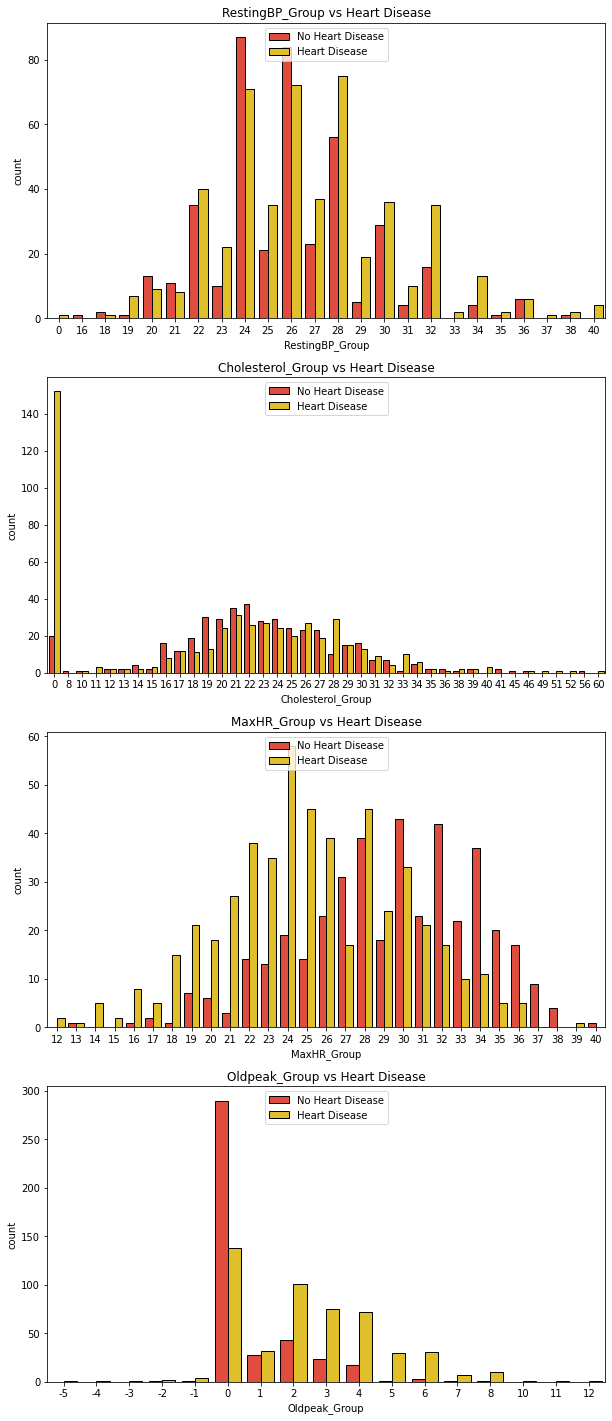
\includegraphics[width=0.5\linewidth]{Figures/Outputs/num-tar-var2.png}
    \label{Comparison between numerical features against average true cases of heart diseases}
    \caption{Comparison of numerical features against average positive cases of heart diseases.}
\end{figure}
\subsection*{Observations}
\begin{itemize}
    \item From the \textbf{RestingBP} group data, \textbf{95} (19x5) - \textbf{170} (34x5) readings are most prone to be detected with heart diseases.
    \item \textbf{Cholesterol} levels between \textbf{160} (16x10) - \textbf{340} (34x10) are highly susceptible to heart diseases.
    \item For the \textbf{MaxHR} readings, heart diseases are found throughout the data but \textbf{70} (14x5) -\textbf{180} (36x5) values has detected many cases. 
    \item \textbf{Oldpeak} values also display heart diseases throughout. \textbf{0} (0x5/10) - \textbf{4} (8x5/10) slope values display high probability to be diagnosed with heart diseases.
\end{itemize}

\section{Numerical features against Categorical features w.r.t Target variable}
\subsection{How does sex influence Numerical Features?}
\begin{figure}[!htpb]
    \centering
    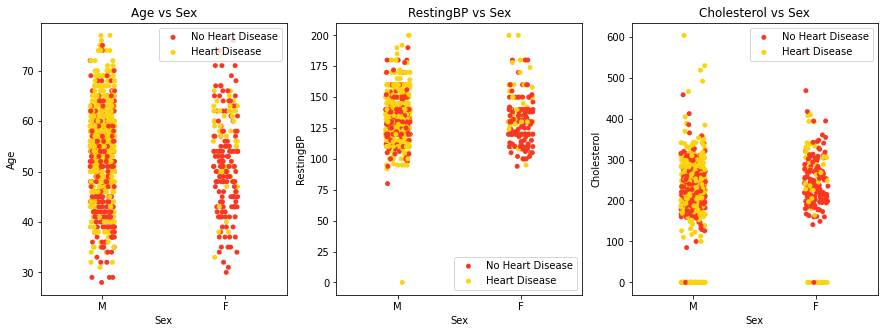
\includegraphics[width=0.7\linewidth]{Figures/Outputs/sex-num-fea.png}
    \label{Comparison between numerical features against gender}
    \caption{Comparison of numerical features against gender.}
\end{figure}
\begin{figure}[!htpb]
    \centering
    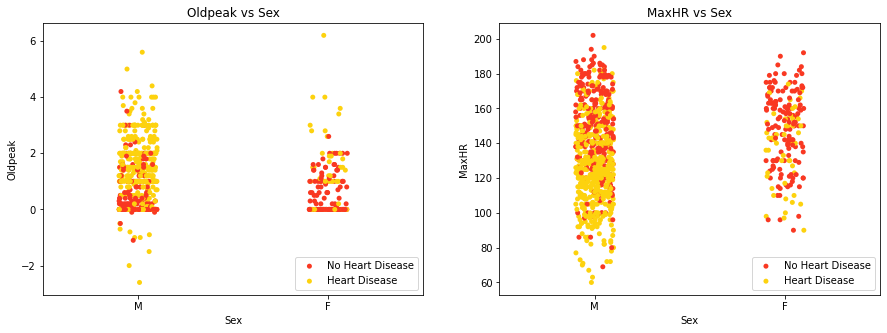
\includegraphics[width=0.7\linewidth]{Figures/Outputs/sex-num-fea2.png}
    \label{Comparison between numerical features against gender}
    \caption{Comparison of numerical features against gender.}
\end{figure}
\begin{itemize}
    \item \textbf{Male} population displays heart diseases at near about all the values of the numerical features. Above the age of 50, positive old peak values and maximum heart rate below 140, heart diseases in male population become dense.
    \item \textbf{Female} population data points are very less as compared to \textbf{male} population data points. Hence, we cannot point to specific ranges or values that display cases of heart diseases. 
\end{itemize}

\subsection{How does Chest Pain Type compare against Numerical features?}
\begin{figure}[!htpb]
    \centering
    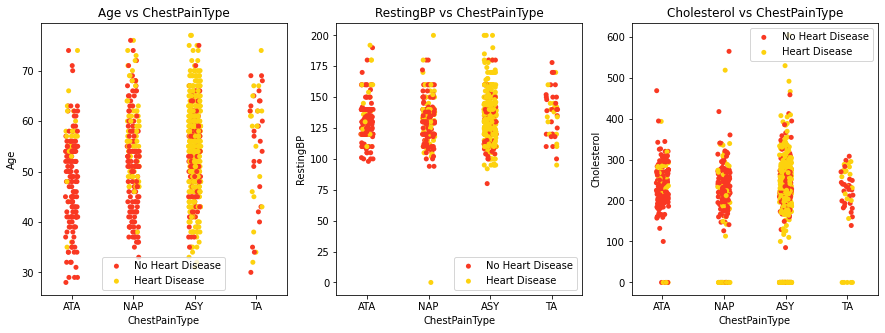
\includegraphics[width=0.7\linewidth]{Figures/Outputs/ches-num.png}
    \label{Comparison between numerical features against chest pain type}
    \caption{Comparison of numerical features against chest pain type.}
\end{figure}
\begin{figure}[!htpb]
    \centering
    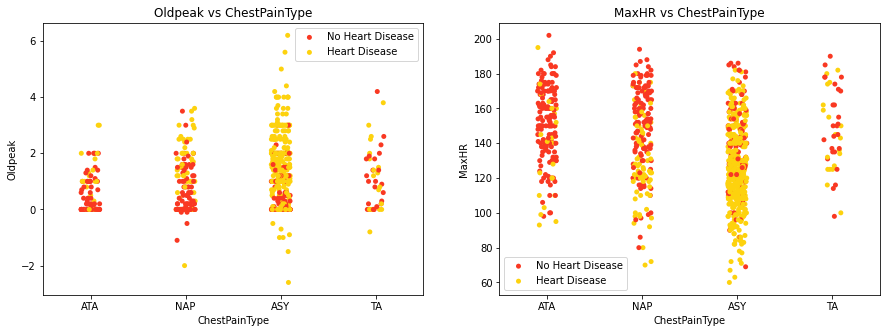
\includegraphics[width=0.7\linewidth]{Figures/Outputs/ches-num2.png}
    \label{Comparison between numerical features against chest pain type.}
    \caption{Comparison of numerical features against chest pain type.}
\end{figure}
\textbf{ASY type of chest pain dominates other types of chest pain in all the numerical features by a lot.}

\subsection{How does FastingBS influence the numerical features?}
\begin{figure}[!htpb]
    \centering
    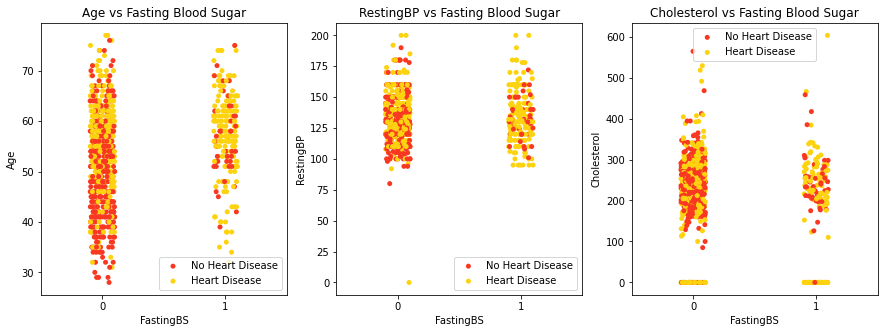
\includegraphics[width=0.7\linewidth]{Figures/Outputs/fasting-num.png}
    \label{Comparison between numerical features against FastingBS}
    \caption{Comparison of numerical features against FastingBS.}
\end{figure}
\begin{figure}[!htpb]
    \centering
    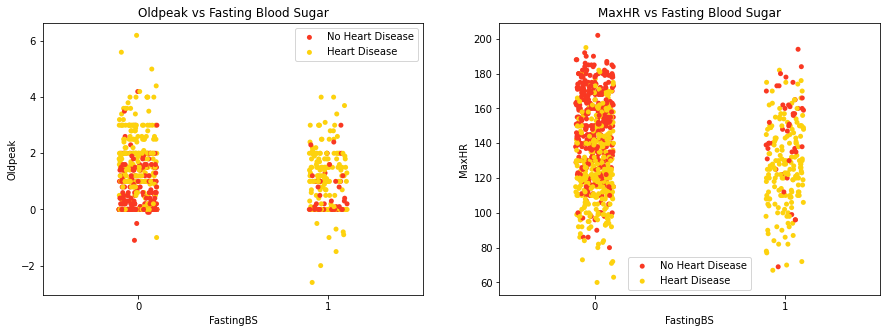
\includegraphics[width=0.7\linewidth]{Figures/Outputs/fasting-num2.png}
    \label{Comparison between numerical features against FastingBS.}
    \caption{Comparison of numerical features against FastingBS.}
\end{figure}
\begin{itemize}
    \item Above the \textbf{age} 50, heart diseases are found throughout the data irrespective of the patient being diagnosed with Fasting Blood Sugar or not.
    \item \textbf{Fasting Blood Sugar} with \textbf{Resting BP} over 100 has displayed more cases of heart diseases than patients with no fasting blood sugar.
    \item \textbf{Cholesterol} with \textbf{Fasting Blood Sugar} does not seem to have an effect in understanding reason behind heart diseases.
    \item Patients that have not been found positive with \textbf{Fasting Blood Sugar} but have maximum heart rate below 130 are more prone to heart diseases.
\end{itemize}

\subsection{How does RestingECG influence the numerical features?}
\begin{figure}[!htpb]
    \centering
    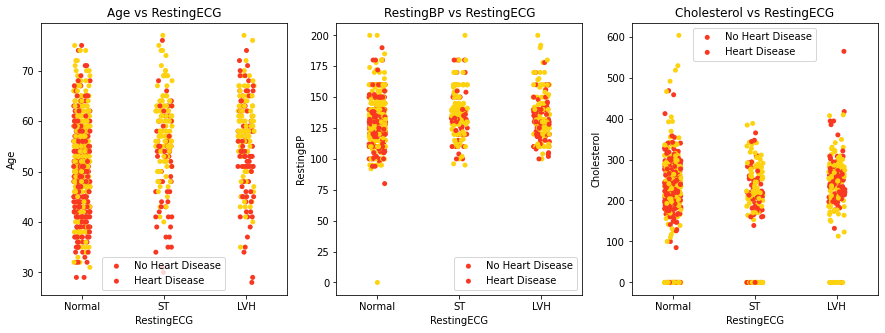
\includegraphics[width=0.7\linewidth]{Figures/Outputs/resting-num.png}
    \label{Comparison between numerical features against RestingECG}
    \caption{Comparison of numerical features against RestingECG.}
\end{figure}
\begin{figure}[!htpb]
    \centering
    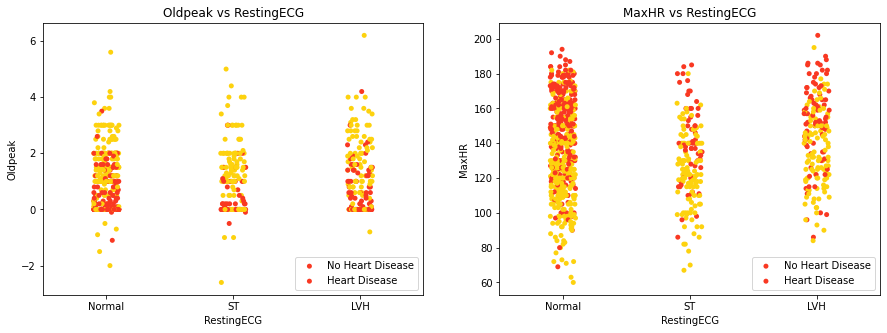
\includegraphics[width=0.7\linewidth]{Figures/Outputs/resting-num2.png}
    \label{Comparison between numerical features against RestingECG}
    \caption{Comparison of numerical features against RestingECG.}
\end{figure}
\begin{itemize}
    \item Heart diseases with \textbf{RestingECG} values of \textbf{Normal}, \textbf{ST} and \textbf{LVH} are detected starting from 30,40 and 40 respectively. Patients above the age of 50 are more prone than any other ages irrespective of \textbf{RestingECG} values.
    \item Heart diseases are found consistently throughout any values of \textbf{RestingBP} and \textbf{RestingECG}.
    \item \textbf{Cholesterol} values between 200 - 300 coupled with \textbf{ST} value of \textbf{RestingECG} display a patch of patients suffering from heart diseases. 
    \item For \textbf{maximum Heart Rate} values, heart diseases are detected in dense below 140 points and \textbf{Normal} RestingECG. \textbf{ST} and \textbf{LVH} throughout the maximum heart rate values display heart disease cases.
\end{itemize}

\subsection{How does ExcerciseAngina influence the numerical features?}
\begin{figure}[!htpb]
    \centering
    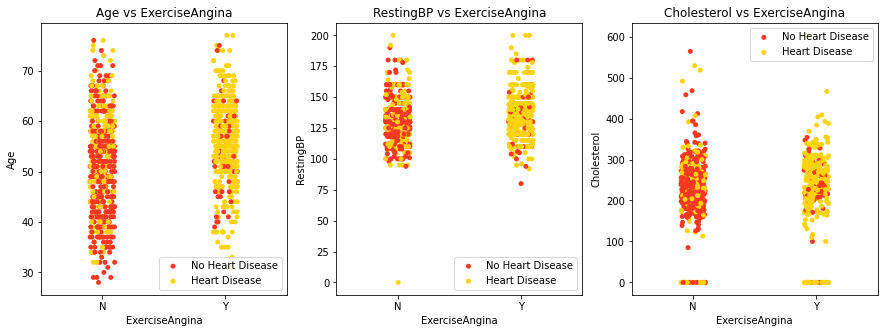
\includegraphics[width=0.7\linewidth]{Figures/Outputs/exer-ang.png}
    \label{Comparison between numerical features against ExerciseAngina}
    \caption{Comparison of numerical features against ExerciseAngina.}
\end{figure}
\begin{figure}[!htpb]
    \centering
    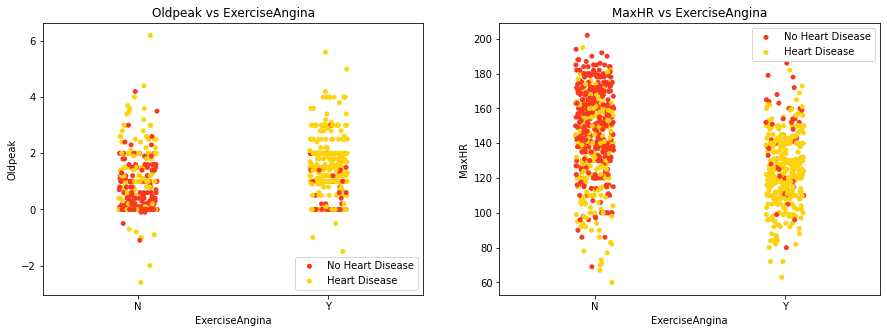
\includegraphics[width=0.7\linewidth]{Figures/Outputs/exer-ang2.png}
    \label{Comparison between numerical features against ExerciseAngina}
    \caption{Comparison of numerical features against ExerciseAngina.}
\end{figure}
A crystal clear observation can be made about the relationship between \textbf{heart disease} case and \textbf{Exercise induced Angina}. A positive correlation between the 2 features can be concluded throughout all the numerical features. 
\newpage
\subsection{How does ST\_Slope influence the numerical features?}
\begin{figure}[!htpb]
    \centering
    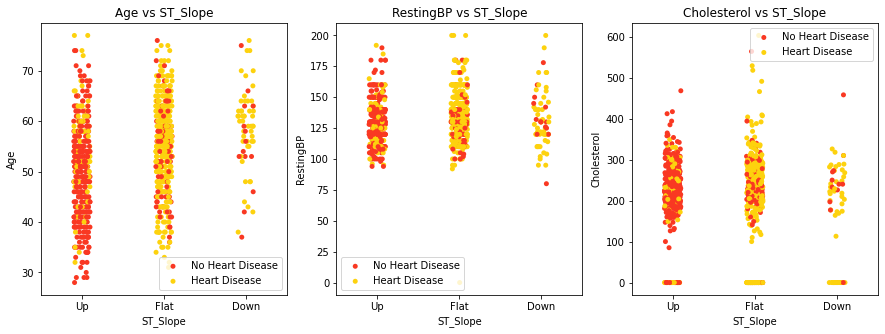
\includegraphics[width=0.7\linewidth]{Figures/Outputs/stslope-num.png}
    \label{Comparison between numerical features against ST_Slope}
    \caption{Comparison of numerical features against ST\_Slope.}
\end{figure}
\begin{figure}[!htpb]
    \centering
    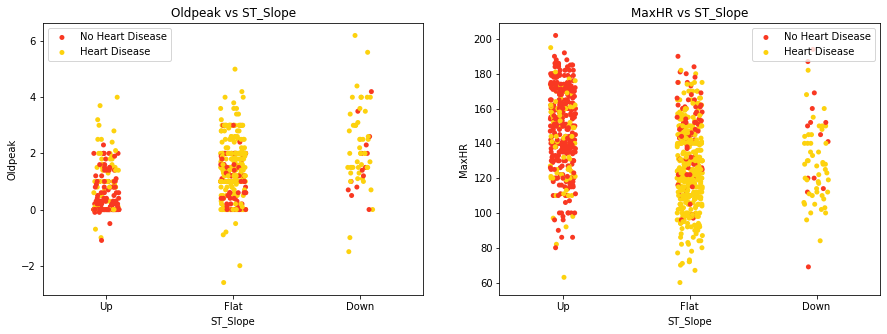
\includegraphics[width=0.7\linewidth]{Figures/Outputs/stslope-num2.png}
    \label{Comparison between numerical features against ST_Slope}
    \caption{Comparison of numerical features against ST\_Slope.}
\end{figure}
\begin{itemize}
    \item Another crystal clear positive observation can be made about the positive correlation between \textbf{ST\_Slope} value and \textbf{Heart Disease} cases. 
    \item \textbf{Flat}, \textbf{Down} and \textbf{Up} in that order display high, middle and low probability of being diagnosed with heart diseases respectively.
\end{itemize}
\newpage
\section{Influence of numerical features by the other numerical features w.r.t target variables}
\begin{figure}[!htpb]
    \centering
    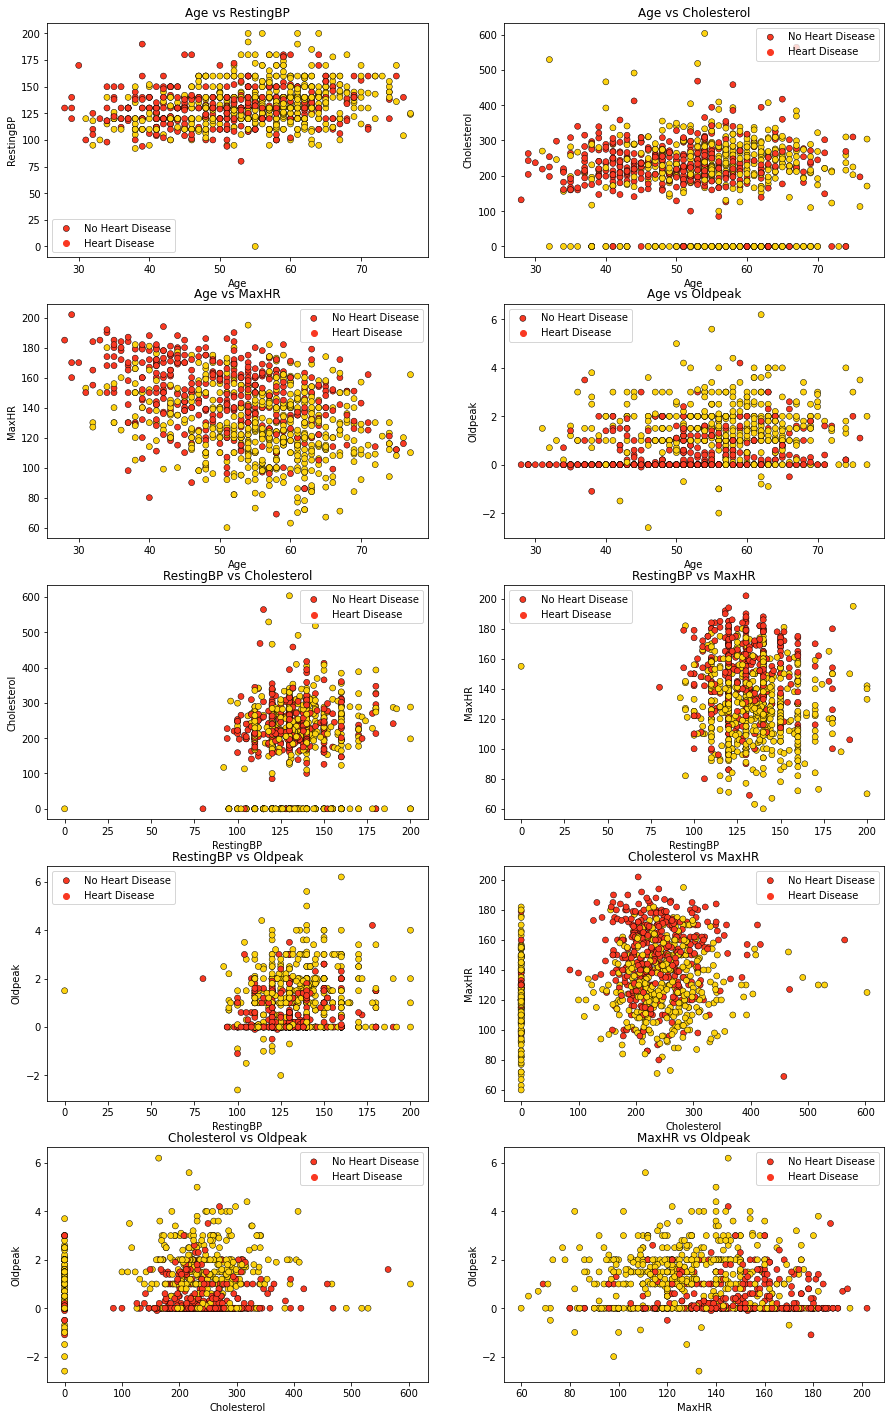
\includegraphics[width=0.7\linewidth]{Figures/Outputs/numf-numf.png}
    \label{Comparison between numerical features against other numerical features}
    \caption{Comparison of numerical features against other numerical features.}
\end{figure}
\subsection*{Conclusions}
\begin{itemize}
    \item - For \textbf{age} 50+, \textbf{RestingBP}* between 100 - 175, \textbf{Cholesterol} level of 200 - 300,\textbf{Max Heart Rate}* below 160 and positive \textbf{oldpeak} values displays high cases of heart disease.
    \item For \textbf{RestingBP} values 100 - 175, highlights too many heart disease patients for all the features.
    \item \textbf{Cholesterol} values 200 - 300 dominates the heart disease cases.
    \item Similarly, \textbf{Max Heart Rate} values below 140 has high probability of being diagnosed with heart diseases.
\end{itemize}

\section{Summary of the observations}
Now with the help of the above observations we may find the order of increasing risk of heart failures due to the studied features:
\begin{itemize}
    \item \textbf{Categorical features}:
    \begin{enumerate}
        \item Sex : Male > Female
        \item ChestPainType : ASY > NAP > ATA > TA
        \item FastingBS : ( FBS < 120 mg/dl ) > ( FBS > 120 mg/dl)
        \item RestingECG : Normal > ST > LVH
        \item ExerciseAngina : Angina > No Angina
        \item ST\_Slope : Flat > Up > Down
    \end{enumerate}
    \item \textbf{Numerical features}:
    \begin{enumerate}
        \item Age : 50+
        \item RestingBP : 95 - 170 
        \item Cholesterol : 160 - 340
        \item MaxHR : 70 - 180
        \item Oldpeak : 0 - 4
    \end{enumerate}
\end{itemize}
\textbf{Now that we have understood the typical values of the features, we may move on to the next step where we select the appropriate features for modeling.}